In this section, we explain in detail our encoding of the UC security definition into Nomos-UC.
Recall from Section~\ref{sec:background} that the UC security definition $\F_1 \xrightarrow{\pi} \F_2$ says we can realize some desired application $\F_2$ with a protocol $\pi$ that uses $\F_1$.
More generally, we define UC realization in terms of an indistinguishability relation between two experiments, the real-world featuring the execution of $\pi$ with $\F_1$, and an ideal-world execution of $\F_2$ and an ideal protocol $\idealP$ that just relays inputs/outputs directly to/from $\F_2$.%
\footnote{This ideal protocol $\idealP$ is also the identity, since we can easily show $\F \xrightarrow{\idealP} \F$ for any functionality $\F$.}
Below, we introduce how the UC experiment is implemented in NomosUC, and then provide a composition operator $\circ$ for protocols, and one for simulators, that satisfies Theorem~\ref{thm:singlecomp}.

\subsection{The UC Experiment}
The UC experiment is an execution of protocol parties and an ideal functionality, reacting to input by an adversary \A or the environment \Z.
We define the \inline{execUC}, in Figure~\ref{lst:execuc}, process as the initial process in the configuration, and it spawns the main processes in the execution: a environment \Z, a \partywrapper, an adversary \A, and a functionality \F.
Its type parameters are all of the message types, import amounts used in the protocol, and some number of token types depending on the protocol in question. In the example in Figure~\ref{fig:execuc} we show \inline{execUC} where some processes, like the simulator for commitments, will need a virtual token type \inline{K1}.
Its function parameters are only the security parameter \inline{k} and a soure of randomnes \inline{rng} that it multiplexes to the rest of the execution. 
The Nomos language currently doesn't support passing proceses definition as paramters, so \inline{execUC} imports a user-defined library \inline{PS} that defines processes for each part of the execution.

NomosUC relies on providerless channels so \inline{execUC} first spawns the communicators that all the shell processes will communicate over.
For example, the channel between \Z and \A is instantiated as 
\begin{lstlisting}[basicstyle=\footnotesize\BeraMonottFamily, mathescape]
#z_to_a $\leftarrow$ communicator_init[$\tp{K}$][$\tp{z2a}$]{$\tp{z2an}$}
#a_to_z $\leftarrow$ communicator_init[$\tp{K}$][$\tp{a2z}$]{$\tp{a2zn}$}
\end{lstlisting}
where the type of \inline{#z_to_a} is given in Section~\ref{subsec:communicators}.
Ultimately the shell processes will attempt to read messages from the shared channels and shuttle them to their internal processes which makes use of session types.

The environment \Z must be the first processes that is spawned because it determines the currptiion set \inline{clist : [PID]} and the session ID (type defined by the user) for the execution (see session type \msg{EtoZ} below).
It accepts its communicators to the \partywrapper and \A and type parameters for the token types it expects to use. 
The session type of \Z forms the basis of the indistinguishability definition later in this section.
{\centering
\parbox{0cm}{
\begin{tabbing}
 $\m{EtoZ}[a] = \up \ichoice{\mb{init}: $\=$ a \arrow [PID] \arrow$ \\
\>$\echoice{\mb{start} \arrow \ichoice{\mb{bit}: Bit \arrow 1}}}$
 \end{tabbing}}
}
The environment concludes the execution by outputting a bit as its guess of whether it's in the real or ideal world. 
When we define indistinguishability, we want the distribution of output bits to be as close to coin tossing as possible (different with negligible probability).
%Sandboxing is a common design pattern in UC, especially for simulators.
%NomosUC supports it through the use of virtual tokens, however, the statically typed nature of NomosUC requires us to be explicit about the number of virtual tokens in use in an execution.
%Therefore, we are unable to pass in a variable number of virtual token types to \inline{execUC}, and must rely on generating simple code to declare \inline{execUC} with a sufficient number of type parameters.
%For example, an execution where the simulator sandboxes the real world adversary, \inline{execUC} will require at least one virtual token type referenced by \inline{K1} in the following definition:

%\begin{figure*}[t]
%\begin{lstlisting}[basicstyle=\scriptsize\BeraMonottFamily, frame=single, mathescape, caption={The process definition of the \msf{execUC} function.}]
%$\Stype$ Bit{n} = <{n}| &{ exec: +{out : Bit $\rightarrow$ 1}} ;
%
%$\tb{proc}$ execUC[$\tp{K}$][$\tp{K1}$][$\tp{sid}$][$\tp{p2f,f2p}$][$\tp{z2p,p2z}$][$\tp{a2p,p2a}$][$\tp{a2f,f2a}$]{$\tp{p2fn,f2pn}$}{$\tp{p2zn,z2pn}$}{$\tp{a2pn,p2an}$}{$\tp{a2fn,f2an}$} :
%  (k: $\tgr{int}$), (r: [Bit]) |- ($\$$d: Bit)
%\end{lstlisting}
%\label{lst:execuc}
%\end{figure*}

%In general, as we will discuss when introducing the \partywrapper, an execution always requires at least one virtual token type.

%\paragraph*{\textbf{The Environment}}
%The environment is the first machine that \inline{execUC} spawns and receives from it the session id and list of corrupted parties for this execution. 
%It can be considered the \emph{first} ITM in the execution.
%Its role in the execution is specified by the type \inline{EtoZ} of the channel it offers.
%\begin{lstlisting}[basicstyle=\scriptsize\BeraMonottFamily, mathescape, frame=single]
%$\Type$ EtoZ[$\tp{a}$] = +{init: a ^ list[$\tp{pid}$] -> exec} 
%$\Type$ exec = &{start : output_bit} ;
%$\Type$ output_bit = +{bit: Bit -> 1} ;
%
%$\tb{proc}$ PS.env[$\tp{K}$][$\tp{z2p,...}$]{$\tp{p2zn,...}$} : 
%  (k: $\tgr{int}$), (r: [Bit]), (#ztop: comm[$\tp{z2pmsg[z2p]]{z2pn}}$), 
%  (#ptoz: comm[$\tp{p2zmsg[p2z]]{p2zn}}$)...  |- ($\$$z : EtoZ) $\tg{(* <- offered channel *)}$
%\end{lstlisting}
%\inline{EtoZ} reflects that the environment must first determine the session id, or \inline{sid}, of the execution as well as which parties it wants to statically corrupt in the form of a \inline{list} of \inline{pid}s.
%Finally, it is told to start and eventually returns an output \inline{bit} indicating it's guess as to whether it's in the real world or the ideal world.
%This output bit, and the environment's decision function, go on to define emulation and indistinguishability later in this section. 
%
%The remainder of the main processes of \inline{execUC} are typed very similarly: they accept channels relevant to them, accept all the other same parameters, and don't offer a channel.

\paragraph*{\textbf{Ideal Functionalities}}
\todo{the point here is to highlight what ideal functionalities look like in NomosUC not just an example that is a tradeoff.}
The core of the UC framework is the ideal functionality: it captures all of the desired security properties in a simple trusted third party.
We use the 2-way channel ideal functionality, \Fauth, as an illustration of some of the limits of session types and design tradeoffs that need to be considered.
The functionality allows two parties to send messages to each other with \A determining when messages are delievered.
From the point of view of either part $P_i$, it can write to \Fauth or receive a message from it---a communication pattern that can't be expressed by a single session type.
Most functionalities that exhibit ambiguity in which end point can send a message must fallback on two competing approaches: split communication over two uni-directional channels or switch communication to polling where the party or \A asks \Fauth for new messages.
Both cases can be captured by session types but lose some of the power of the session type mediating the order of messages in the protocol. 
For example int he former approach the session types for \Fauth look something like this

%We use providerless channels, in part, to allow functionalities in NomosUC to use meaningful session types with a dynamic number of parties.
%The 2-way channel ideal functionality, \Fauth, is a simple and clear illustration of design choices and tradeoffs when writing functionalities in NomosUC.
%\Fauth provides only message \emph{integrity} and leaks the message to \A.
%When a message is sent by $P_s$, \Fauth sends the message to \A and waits for a response to deliver it to $P_r$. 
%
%In plain session types, communication between two parties $P_s$ and $P_r$ occurs over a single duplex channel.
%In UC the role of the adversary as a message scheduler in \Fauth, the most common network channel model, means a more complicated functionality involving $P_s$, $P_r$, \F, and \A. 
%\Fauth provides only the following guarantee: (\emph{integrity}) the adversary can not modify messages from the sender.
%It sends the message to \A when it receives one from the sender, and waits for the adversary to instruct it to deliver the message.
%When \A writes back to \Fauth to deliver the message, \Fauth sends it to the receiver.
%The communication pattern in \Fauth exhibits the same problems with the communication in Figure~\ref{fig:newpandq}.
%
%We, therefore, are confronted with two options: transition to a functionality where all parties and the adversary poll for new messages or split communication among two uni-directional providerless channels.
%The former buffers messages from $P_s$ until asked for by $A$, and then delivers (with \A's approval) to $P_r$ when polled.
%The type and mechanics of this version require constant activations by \Z and are inconvenient.
%The latter is a more generalizable construction and can be typed as: 
\begin{center}
\parbox{0cm}{
\begin{tabbing}
$\m{sendmsg}[a] = \textcolor{red}{\getpot^n} \ichoice{\mb{send}: \m{a} \product \m{sendmsg}}$ \\
$\m{recvmsg}[a] = \textcolor{red}{\getpot^m} \echoice{\mb{recv}: \m{a} \product \m{recvmsg}}$ \\
$\m{adv}[a] = \echoice{\mb{leakmsg}: a \product \ichoice{ \mb{ok}: \m{adv}}}$
\end{tabbing}}
\end{center}
where each party has one channel typed as $\m{sending}$ and the other as $\m{recvmsg}$.
Despite this limitation we note that the type parameter $a$ for the message type ensures that no party can receice a message from \Fauth before a message is sent which concretizes $a$ to some type.
Therefore, although some of the power of session types is lost when dealing with such functionalities, they are still capable of enforcing protocol message ordering and providing resource analysis through import.

\subsection{The \partywrapper}
\begin{figure}
	\centering
	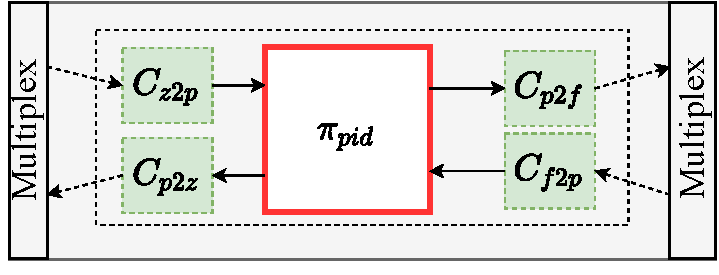
\includegraphics[scale=0.5]{figures/singleshellmultiplex.pdf}
	\caption{This is the \partywrapper that routes messages to the correct internally runnint protocol party. This figure shows how one protoco party (dotted box) is instantiated within it. The party $\pi_{pid}$ is shell code akin to Figure~\ref{fig:newpandq}.}%\snote{Updated caption to say it's multiplexer with one instance. The reason I don't want to include another instance is that I couldn't figure out a way to add it and expand the diagram horizontally. It will leave so much white space on the sides if I add a new party and will take up much more vertical space which we need to cut down on anyway.}}
	\label{fig:singlemultiplex}
	\vspace{-3mm}
\end{figure}
The \partywrapper is a programming construct created to make it easy to manage a dynamic set of protocol parties. 
%Without the \partywrapper, NomosUC may have to rely on \Z to create the channels for new parties and route messages to them.
%Similarly, \F and \A would have to all handle new channels from the creation of new parties.
The \partywrapper runs all of the protocol parties internally in a sandbox, has one providerless channel to \Z, one to \A, and one with \F, and it multiplexes messages to and from them to its internal parties. 
The \partywrapper is not a requirement specific to the session-typed setting of NomosUC, but motivated by the use of channels for communication.

The \partywrapper spawns parties internally with virtual providerless channels so that some party $\pi_i$ sees an interface for communicating with \F and \Z as if it were a real process.
In actuality, the \partywrapper is connected to \Z via communicator whose type includes the $\m{PID}$ with every message, and it routes messages to the appropriate virtual instance.
An example of a party $\pi_i$ running within the \partywrapper is shown in Figure~\ref{fig:singlemultiplex}. The process $\pi_{pid}$ is the shell process mentioned previously and is connected to communicators as expected from providerless channels. The endpoint of the communicators is the \partywrapper.  

This construction affects the import sent from \Z to a protocol party. With distinct, real parties \Z sends differing amounts of import to each party depending on its session type.
Now, the single communicator forces \Z to always send the same import with every message to $\pi$ and receive some constrant amount on incoming messages.
This extends to messages between the \partywrapper and \F as well.
%Despite this constraint, it is easy to define import in such a way by taking the maximum required over all possible messages between \Z and some $\pi$.

In our quest to meaningfully apply session types to ideal functionalities, we are left with \F having one shared channel to the \partywrapper and losing the heart and soul of session types.
We overcome this by replicating what happens in the \partywrapper as a shell around the ideal functionality.
Similar to the \partywrapper, the shell around \F also presents virtual providerless channels as an interface to the underlying \F. This ensures that session types can meaningfully express protocol message ordeirng and import requirements while enabling dynamic party management. 

%
%The environment must communicate with multiple parties and needs multiple channels to do so. 
%Forcing \Z to handle creating new providerless channels to new parties is an inefficient design.
%If we simplify to a single channel and multiplex, the statically-typed nature of the session type means only a static number of parties can be specified. 
%NomosUC overcomes these constraints by using a \partywrapper to encapsulate all protocol parties and run them internally.
%We use the notation \m{MX}(\PI) to denote the \partywrapper running parties of protocol \PI.
%
%The purpose of the \partywrapper is to support a dynamic set of parties without \Z, \A, or \F having to react to new parties and manage a growing set of channels.
%Instead, the \partywrapper acts as singular endpoint for all communication with protocol parties, and it manages the creation of new parties and routing messages to/from them.
%
%Furthermore, it are connected to \Z, \A, and \F through providerless channels (Section~\ref{sec:basic}).
%From the point of view of parties running inside the \partywrapper, they are directly connected to \F and \Z in the way of Figure~\ref{fig:newpandq}.
%The shell code around each party offers four channels, two for each providerless connection, with \F and with \Z, with the appropriate session types. 
%For commitment and communication with \Z, the shell code offers channels with type \m{sender} or \m{receiver}, and the type of \Fro, which we examine later, for communication with \F~\footnote{\Fcom and \Fro make use of only one of their channels to parties instead of both.}.
%However, because we run parties of \PI internal to the \partywrapper, it runs instances of the shell code for each new spawned party and creates communicators around it that it can write/read pid-specific messages to/from.
%Figure~\ref{fig:singlemultiplex} illustrates how the shell code $\pi_{pid}$ is connected to communicators for each direction. This construction is repeated for every new party spawned inside the \partywrapper.
%
%\paragraph{Import with the \partywrapper}
%Virtualizing protocol parties in the \partywrapper means that they all, effectively, share the same \emph{real} import and potential, even though they are given virtual potential.
%We reason that the \partywrapper does not change the import requirements of protocols or make some protocols unrealizable in NomosUC.
%Mainly, for any activation of a party, the party either retains some import or gives away all the import it receives. 
%The former case allows parties to do polynomial work or be activated a polynomial number of times, and the latter case allows for parties activated a constant number of times, doing constant work per activation.
%The \partywrapper alone does constant work per activation, therefore, in either case both the protocol party and \partywrapper have enough import to perform their necessary computations.

%\paragraph*{\textbf{The Adversary}}
%Since the adversary is arbitrary unlike protocols and functionalities, it is does not directly use session-types in NomosUC and receives inputs from \Z in the form of functional messages only.

\subsection{Polynomial Bound}
The UC framework introduces the concept of import tokens as a new way to reason about ITMs being polynomial in the security parameter $k$. 
The import mechainsm as described in UC, and which we describe in Section~\ref{sec:background}, ensures that a single ITM's execution is upper-bounded by some poynomial $T(n,k)$ where $T$ is a polynomial, $n$ is its net import token balance (received - sent), and $k$ is the security parameter.
%Canetti et al. limit their discussion to parameterized systems where no machine does anything until it's received at least $k$ import.
%We depart from this notion slightly and express ``interactive polynomial time'' by using a bounding polynomial in both import and $k$.
%We do this for two reasons.
%First, it allows us to reason directly about processes being polynomia in $k$ without including the extra notion of ``paraeterized sytems'' in UC.
%Second, adding $k$ to the polynomial makes our definitions of import requirements for functionalities, like \Fro, more intuitive by requiring only 1 unit of import for one-time poynomial computations.

In Section~\ref{sec:import}, we described how the NomosUC type systems judges processes to be PPT in the security parameter $k$. 
It still remains to show the soundness of our import definition by extending the local polynomial guarantee to show that the UC experiment is PPT in $k$.
%In NomosUC, we build import into the type system.
%Specifically, the system provides novel constructs to exchange import, generate potential from that import, and create virtual import for virtualization and cryptographic reductions.
%The language additionally encodes the computational cost of each operation performed by an ITM, and statically guarantees that the execution cost of each ITM is locally polynomial in the net import it has over its entire execution. 
%Therefore, our type system subsumes the need to reason that our handling of polynomial time can judge local polynomial time.
%Instead, in this section, show the soundness of our import definition by extending the local polynomial guarantee to show that the entire UC experiment is PPT in the security parameter $k$.

%We first define what it means to be PPT for a process, or term, in NomosUC. 
%\todo{experimental addition of the $\leq$ in the definition below, unclear if that is a good decision}
\begin{ddef}[PPT in $k$]\label{def:ppt}
A closed term $e(k,r)$ is  PPT in the $k$ if, given some amount of initial import $n$ polynomial in $k$, there exists a polynomial $T(n,k)$ such that $\forall k, r, e(r,k) \{n\}$ terminates in at most $T(n,k)$ steps.
We use the notation $e(r,k) \leq T(n,k)$ to refer to such a PPT process.
\end{ddef}
%Notice that our choice of polynomial representation, a function of both the import and security parameter $k$, only partially defines PPT in terms of the security parameter. It still remains to be shown that the system is polynomial \emph{only} in $k$.

The soundness of our polytime notion comes down to showing that our UC experiment is PPT in only the security parameter $k$. 
%The UC framework provides a simulation of a configuration of ITMs on a universal turing machine and proves that such a turing machine is also bounded by a polynomial $T$. 
%Given the initial input of import tokens into the machine ($poly(k)$ amount of import), it concludes that the import mechanism falls in line with the standard length-of-input notion of polynomial time and satisfied their ``PPT in $k$'' definition. 
In NomosUC, we do not deal directly with ITMs, however, our type system allows us to judge whether a process, or collection of processes through the Preservation Theorem~\ref{thm:preservation}, is locally PPT given a particular polynomial. 
We rely on the Lemma~\ref{lem:local_ppt} and Theorem~\ref{thm:global_ppt} to adapt Proposition 7 from UC~\cite{canettiUC} to NomosUC, and show that our notion of locally PPT leads to a UC execution that is PPT in the security parameter $k$.

In order to reason about configurations in Theorem~\ref{thm:soundness}, we define the UC execution as a series of configurations that capture the relevant processes--the \partywrapper, \Z, \F, and \A--and the channels that connect them.

\begin{theorem} \label{thm:soundness}
Let \F, \A, \Z, and \m{MX}(\PI) be locally PPT configurations bounded by super additive polynomials $T_\F$, $T_\A$, $T_\Z$, $T_\PI$. Let \m{UC} be a configuration composed of a single process that runs \inline{execUC}. If \m{UC} receives $n \in poly(k)$ import initially, then any composed configuration $\m{UC} = \m{execUC} \; || \; \Z \; || \; \A \; || \; \m{MX}(\PI) \; || \; \F$ is PPT in $k$, where \m{MX} is the \partywrapper.
\end{theorem}

\begin{proof}
The resulting configuration \m{UC} has only one channel in it's context: the channel offered by \inline{execUC} of type \inline{Bit}. 
\inline{execUC}, therefore, is the intial process in the configuration and receives the intial import $n \in poly(k)$.

By the \m{compose} rule, the Preservation Theorem~\ref{thm:preservation}, and Theorem~\ref{thm:global_ppt} the work done by the resulting configuration is strictly the sum of the work done by the composed configurations, and the resulting configuration \m{UC} must also be PPT with some polynomial $T(n,k)$.

If we take the initial import $n$ to be polynomial in $k$, ten we cn conclude that \m{UC} is PPT in $k$ in the traditional length-of-input sense as well.

\end{proof}


\subsection{Emulation}
The central security definition in UC is indistinguishability between the real and ideal world experiments.
In NomosUC, we must be more careful to only consider protocols and adversaries whose types (both message and import) match over the channels they share. 
Therefore, we introduce the term \textit{well-matched} to mean a PPT term $e$ is well-typed when connected to another term $e'$.
Simply put, we want to capture terms $e$ and $e'$ that can be connected over the channels they share.
We use the notation $e \leftrightarrow e'$ to denote well-matched. For the sake of space we present a more precise Definition~\ref{def:wellmatched} in the Appendix. 
%The resulting terms in Definition~\ref{def:wellmatched} are partially closed after connection: the terms may only be connected on some subset of their channels.

%In the UC security definition, we say that a protocol $\pi$ possesses the same security properties as another protocol $\phi$ if no environment can distinguish between them for any adversary.
%In most cases we compare a real protocol $\pi$ with an ideal functionality \F running with ideal parties \idealP.
%They are much simpler than protocols because they don't require any special code to handle mutually distrustful other processes, and they perform the given computation on behald of the ideal world parties.

We define the output bit of the partial term of \inline{execUC}, for a specific $\pi$ and \F, as an ensemble of distributions over all possible random bitstrings and security parameters.
Emulation, then, is about the ensembles created by two UC executions being computationally indistinguishable from each other.
We define indistinuishability between ensembles in a standard way using \textit{statistical distance} in Definition~\ref{def:distance}.

\begin{definition}[Indistinguishability]\label{def:distance}
Two ensembles $\mathcal{D}_{1,k}, \mathcal{D}_{2,k}$ are indistinguishable, $\mathcal{D}_{1,k} \sim \mathcal{D}_{2,k}$, if their statistical distance is at most $negl(k), \forall k$.
\end{definition}

%\paragraph{Validity}
%For the remainder of this section we refer to \emph{valid} adversaries and simulators given a particular protocol, functionality, or environment.
%We refer to adversaries that type-check when connected to \Z, \F, or $\Pi$ by \inline{execUC}, and that are \emph{well-matched} as defined above. 
%Indisintiguishability between two protocols is defined as follows (we shorten the communicator type \msf{comm} to \msf{c}):

UC emulation combines the UC execution with indistinguishability resulting in the following NomosUC emulation definition.
\begin{definition}[Emulation]\label{def:emulation}
Given two protocols $(\pi, \F_1), (\phi, \F_2)$, which we refer to only by \PI and $\phi$ in the theorem, that are well-resource-typed, if $\forall \A$ well-matched with \PI, $\exists \Sim$ well-matched with $\phi$ s.t. $\forall \Z$ : $\msf{execUC}(\pi, \F_1, \Z, \A) \approx \msf{execUC}(\phi, \F_2, \Z, \Sim)$:

\begin{mathpar}
	\footnotesize
	\inferrule*[right=emulate]
	{
		\pi : \Delta_1'[\Tokentypes][\mathrm{T}_{\pi}] \semi \phi : \Delta_2'[\Tokentypes][\mathrm{T}_{\phi}] \semi \\
		\forall \A \, | \, \Delta_4[\Tokentypes][\mathrm{T}_{\A}] \vdash \A :: \Delta_4', \langle \A \leftrightarrow \pi \rangle \\
		\Rightarrow \exists \Delta_3[\Tokentypes][\mathrm{T}_{\Sim}] \vdash \Sim_\A :: \Delta_3', \langle \Sim_\A \leftrightarrow \phi \rangle \\
		\Rightarrow \forall \Z  \; \msf{execUC} \ \pi\ \Z\ \F_1\ \A \approx\ \msf{execUC} \ \phi\ \Z\ \F_2\ \Sim_\A
	}
	{
		% EMULATION DEFINITION
		\lambda \A . \Sim_\A \vdash (\pi, \F_1) \sim (\phi, \F_2)
	}
\end{mathpar}
\end{definition}
The emulation definition requires only that the adverasries in question are well-matched with the protocols being emulated, as our type system already ensures PPT in $k$.

With this emuluation definition we complete our description of UC-realization.
If a simulator exists such that emulation holds for $(\pi, \F_1) \sim (\idealP, \F_2)$ then we say that the protocol $\pi$ UC-realized the functionality $\F_2$ in the $\F_1$-hybrid world:
\[
	\F_1 \xrightarrow{\pi} \F_2
\]

%\paragraph{Import for Functionalities}
%The \Fcom example use throughout this work is realized by protocol that uses the random oracle. 
%A natural notion of import should define \Fcom as requiring 0 import because it is one-shot and halts after doing constant amount of work.
%\Fro on the other hand, requires at least 1 unit of import in order to be handle a potentially polynomial mumber of activations as well as reading/writing $k$-bit strings.
%This poses a problem that the ideal world requires 0 import however, the real world requires at least 1 unit of import.
%We resolve this dilemma by defining functionalities as parameteric in the amount of import they require.
%Parametric functionalities do not restrict UC-realization to only those protocols that are as computationally ``efficient'' as the them. In cryptography, it is common for real protocols to be computationally intensive while the ideal functionality they are realizing is trivial, and we want to be able to express such emulation.
%We modify the arrow notation, slightly, to capture that a functionality can realize itself while requiring more import, and use the notation $\F^m$ to denote a functionality parameterized to require $m$ import.
%\[
%	\F_1^m \xrightarrow{\idealP} \F_2^{n \geq m}
%\]
%For the remainder of this work we do not bother import annotations on functionalities and only concern ourselves with the minimum import they require because it is an implementation detail.

%When we talk about emulation, we particularly care about emulation with respect to an ideal protocol $\phi$ which is really just $(\idealP, \F)$ where \idealP is the protocol which forwards all messages to/from \Z and \F.
%We say the protocol $\pi$ (potentially with a hybrid functionality $\F_1$) UC-realizes an ideal functionality $\F_2$ if Definition~\ref{def:emulation} holds for $(\pi, \F_1)$ and  $\phi = (\idealP, \F_2)$

%\begin{definition}[UC-Realize]
%A protocol $\pi$ UC-realized an ideal functionality $\F_1$ if $(\pi, \F_2) \sim (\idealP, \F_1)$ for some $\F_2$.
%
%\begin{mathpar}
%\footnotesize
%\inferrule*[right=UC-Realize]
%{ (\pi, \F_1) \sim (\idealP, \F_2) }
%{ \F_1 \xrightarrow{\pi} \F_2 }
%\end{mathpar}
%\end{definition}

\subsection{Dummy Lemma} \label{sec:dummy}
The dummy lemma is a crucial result in UC that reduces the design space of simulators to just one: the one for the dummy adversary in the real world.
The Lemma presents the construction of a simulator from the \DS for any adversary \A. Our constructed Dummy Lemma simulator uses virtual tokens to simulate \DS and \A internall and route messages between them.
At a high level the Lemma asserts that an execution with \DS and the dummy adversary must work for all environments even those running some \A internally.
If the \A moves from \Z into the real world execution as th real adverasry and the ideal world connected to \DS then the emulation must still hold.
We provide a diagram presenting this construction in the Appendix as well.
%The Lemma states that if a simulator exists for the dummy adversary, called the dummy simulator \DS, then there it easy to construct a simulator for any other adversary \A. 
%The simulator constructed in this lemma uses virtual tokens to internally run \DS and \A.
%
%The intuitiom behind this results rests in the fact that emulation must hold over $\forall \Z$ for a particular \A. 
%Particularly, in the case of \DS and \DummyAdv, emulation holds for a \Z that may be running any other possible \A internally and passing it's output to \DS and \DummyAdv.
%Therefore, constructing a simulator for \A is equivalent to moving it out of the simulation and into the execution, as the adversary in the real world and as part of the simulator, providing input to \DS, in the ideal world.

\begin{theorem}[Dummy Lemma]\label{thm:dummy}
If \ $\exists \DS$ s.t. $ \DA, \DS \vdash \F_2 \xrightarrow{\pi} \F_1$ then $\forall \A \ \exists \Sim_\A$ s.t. $\Sim_{\A} \vdash  \F_2 \xrightarrow{\pi} \F_1)$ 
\end{theorem}

%We give the proof of this lemma in the appendix, however, we provide an intuition for understanding why it is true.
%Simulation w.r.t the dummy simulator works for all environments, even those that could run any potential real-world adversary internally. Such environments, pass input to the adversary, whose output is given to the dummy simulator. 
%The constructed simulator captures the idea of moving the adversary from the environment into the the execution, and the constructed simulator runs the real-world adversary and dummy simulator internally.
%Environment inputs are now passed to the adversary, and the adversary's outputs are passed to the dummy simulator.

%\begin{proof}
%The constructed simulator $\Sim_\A$ internally simulates \DS and \A through a virtual token type $K'$. 
%We describe the simulation pattern below to simulate messages to \DS and \A.
%
%On \inline{Z2A2P} input from \Z on channel \msf{z2a}, \Sim fowards the message to the internal \A with the same type but virtual tokens instead of real ones:
%\begin{lstlisting}[basicstyle=\small\BeraMonottFamily, frame=single,  mathescape, label={lst:sim}]
%msg = $\nrecv$ $\$$z2a ;
%$\nget$ $\$$z2a {z2an : K} ;
%$\tm{withdrawTokens}$ f K K1 z2an ;
%$\nsend$ $\$$a_z2a msg ;
%$\npay$ {z2an : K1} $\$$a_z2a ; 
%\end{lstlisting}
%
%Similarly, on \inline{A2P(pid,msg)} output from \A to a protocol party on channel \msf{a2p}, \Sim sends the message to \DS as input from \Z (type: \inline{Z2A2P(pid, msg)}:
%\begin{lstlisting}[basicstyle=\small\BeraMonottFamily, frame=single,  mathescape]
%pid = $\tb{recv}$ $\$$a_a2p ;
%msg = $\tb{recv}$ $\$$a_a2p ;
%$\tb{get}$ K1 $\$$aa2p {a2pn} ;
%$\tb{send}$ $\$$sd_z2a A2P(pid, msg) ;
%$\npay$ $\$$sd_z2a {z2an : K1} ;
%\end{lstlisting}
%
%$\Sim_\A$ accepts input from \Z and forwards it to the internal \A, which outputs to either the protocol parties or the ideal functionality. 
%\Sim forwards this output to \DS acting as input from the environment  and forward any outputs \DS creates to the intended recipients.
%Our main proof obligation here is to ensure that $\SIM{\A}$ in NomosUC is well-resource-typed for all well-resource-typed \A.
%The $\Sim_\A$ performs constant overhead on the simulattion of \A and \DS. Therefore, a sufficient bounding polynomial on the runtime of $\Sim_\A$ can be given as:
%\[
%T(n) = T_{\A,\DS}(n) + T_{\A,\DS}(n) + O(n)
%\]
%where $T_{\A,\DS}(n)$ is the greater of the two bounding polynomials for \DS and \A evaluated at $n$, and $n$ is the import that \Z sends to \A and \Sim. 
%We must also reason about the use of virtual tokens.
%Given that \A and \DS are well-resource-typed we can conclude that the virtual import tokens generated for activating \A and \DS never exceeds a polynomial in the number of real import tokens received by \Sim. 
%\end{proof}

\subsection{Single Composition}
In this section we present a composition operator for protocols that completes the single composition theorem, Theorem~\ref{thm:singlecomp}.
The composition operator allows replacement of a functioality with a protocol realizing it, and, potentially, any functionality that protocol uses.

Say a protocol $\pi$, using hybrid functionality $\F_1$, realizes functionality $\F_2$. 
For a protocol $\rho$ that uses $\F_2$, replacement of the functionality with $\pi$ means connecting parties of $\rho$ to the corresponding party of $\pi$ within the \partywrapper.

The basic composition operator replicates communication in Figure~\ref{fig:newpandq} and connects parties of \RHO and parties of \PI be means of providerless channels. 
The communicators created by the party wrapper (outside the dotted box in Figure~\ref{fig:replacement}) reflect the type of the new hybrid functionality of \PI.
%This communicator is not shown as we retain the abstract notion given in Fig~\ref{fig:newpandq}.
%Within the \partywrapper, both \RHO and \PI are connected by multiple session-typed channels to \Z and to \F, and those channels connected to generated processes which read communicator messages and ofrward them to/from the party.
%Recall that the shell codes are generated by the UC-executions of each of \RHO and \PI, and the composition operator duplicates their code here.

%In this section we present a simplified composition theorem and a second theorem we call the squash theorem.
%These two theorems combine later in the section to prove the full UC composition theorem as it appears in the UC framework~\cite{uc}.
%
%Briefly the composition operator allows substitution of a functionality for a protocol that realized is. 
%The theorem states that a protocol that uses some functionaliy \F can replace with a protocol $\pi$ that realizes it along with any hybrid functionality $\pi$ uses.
%More specifically, in NomosUC, say a protocol $(\pi, \F_1)$ realizes some functionality $\F_2$.
%A protocol $\rho$ that uses $\F_2$ can replace is with instances of $\pi$ directly connected to the corresponding instances of $\rho$ \emph{within} the protocol wrapper, and the ideal functionality $\F_2$ being replaced by $\F_1$ in the functionality wrapper.

%We highlight first, that our protocol wrapper construction illustrated in \ref{fig:blankpartywrapper}, connects the internal process in that specific way to enable composition.
%Recal that the Nomos language has the concept of clients and providers for a give linear channel. Given to processes, the type of the channel changes depending on which process \emph{offers} the channel, i.e. is the provider, and who is the client.
%The arrows in Figure~\ref{fig:blankpartywrapper} illustrate the \emph{client} $\rightarrow$ \emph{provider} relationship.
%We illustrate how protocol replacement works in NomosUC in Figure~\ref{fig:replacement}.

\begin{figure}
\centering
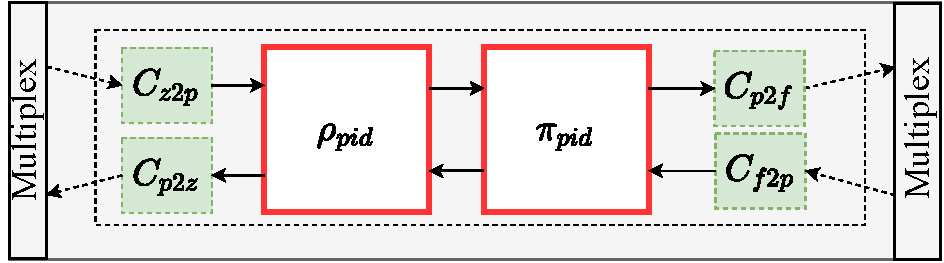
\includegraphics[scale=0.5]{figures/newcompose.pdf}
\caption{When we compose two protocols, we connect the two corresponding parties of each (with the same \m{pid}, in the way of Figure~\ref{fig:newpandq}. The arrows between \RHO and \PI abstract away communicator details. The communicators on the right side of \PI correspond to the type of \PI with it hybrid functionality.}
\label{fig:replacement}
\end{figure}

%The code for the operator has the same type as any other protocol except, from the description above, it's offered channel is for the type of the functionality $\F_1$ instead of $\F_2$.
%We rely on the code generation for to handle spawning instaces of a \inline{p2f} process corresponding to $\pi$ rather than $\rho$.
%The operator is given in Figure~\ref{lst:compose}.
%\begin{figure}
%\begin{lstlisting}[basicstyle=\footnotesize\BeraMonottFamily, frame=single, mathescape]
%$\tb{proc}$ compose[K][z,p]:
%  (pid: Int), (rng: [Bit]), (sid: session[1]),
%  (pid: Int), ($\$$z2p: z) |- ($\$$c: p) =
%{
%  $\$$ch <- PS.rho <- k rng sid pid $\$$z2p ;
%  $\$$c <- Ps.pi <- k rng sid pid $\$$ch 
%}
%\end{lstlisting}
%\caption{The composition operator accepts the same parameters as any other protocol party and offers the channel of type $p2f$ of the realizing protocol $\pi$. We connect $\rho$ to $\pi$ as an environment giving input to $\pi$. We do not need to include any import in our composition operator as the two protocols are guaranteed to be well-matched by the emulation definition. The operator replaces only one party (one \msf{pid}), and the \partywrapper instantiates parties that run the composed protocol.}
%\label{lst:compose}
%\end{figure}

We further require a composition operator for simulators and we briefly describe, in writing, how to connect two sandboxed simulators \SIM{\rho} and \SIM{\pi} inside the construction simulator.
At a high level we connect the simulators in the natural, intuitive way.
Inputs to the adversary are intended for $\F_1$ or dummy parties of $\F_1$ and are handled by \SIM{\pi}. Outputs from \SIM{\pi} are intended for $\F_2$ and dummy parties of $\F_2$ which is simulated by \SIM{\rho}.
Messages from the protocol/functionality to the simulator are similarly sent to \SIM{\rho} first, and its outputs go to \SIM{\pi}.
You can find the full simulator composition operator in the appendix.
%\begin{itemize}
%	\item Input from \Z is split between the two simulators
%	\begin{itemize} 
%		\item \inline{Z2A2P(pid, msg)} intended for parties of $\rho$ are passed to \SIM{\rho}.
%		\item \inline{Z2A2F(msg)} intended for $\F_1$ is passed to \SIM{\pi}.
%	\end{itemize}
%	\item Output from \SIM{\pi}: 
%	\begin{itemize}
%		\item \inline{A2F(msg)} for $\F_2$ and \inline{A2P(pid,msg)} for dummy parties of $\F_2$ are sent to \SIM{\rho} as \inline{Z2A2F(msg)}
%		\item \inline{F2A2Z(msg)} is sent to \Z unaltered with no import (UC dictates no import is sent to \A from either corrupt parties or \F).
%	\end{itemize}
%	\item Output from \SIM{\rho}: 
%	\begin{itemize}
%		\item \inline{A2F(msg)} and \inline{A2P(pid,msg)} for $\F_3$ with $n$ virtual import are sent unaltered with $n$ real import.
%		\item \inline{F2A2Z(msg)} messages are sent to \SIM{\pi} as \inline{F2A(msg)} from $\F_2$.
%		\item \inline{P2A2Z(pid,msg)} messages are sent to \Z unaltered with no import.
%	\end{itemize}
%\end{itemize}
%The simulator relies on simulators for $\F_1 \xrightarrow{\pi} \F_3$ and $\F_2 \xrightarrow{\rho} \F_3$ to satisfy simulation for Theorem~\ref{thm:singlecomp}.
%The simulator performs constant overhead on \SIM{\pi} and \SIM{\rho}, and, therefore, we can conclude that it adheres to the polynomial time notion define by our type system and is well-resource-typed.
%The type in the ideal world gurantees that both the real and ideal world adversaries get at least as much impor as any of the protocol parties. 
%This ensures that the composed simulator has enough import to sandbox the two existing simulators and send import out to the ideal world parties and ideal funfctionality.
%Therefore it is trivial to see that the composed simulator is well-resource-typed.

%An illustrative description of the intuition behind composition is shown by this series of UC executions where the $\equiv$ operator denotes equivalent UC executions that result from moving ITMs in and out of a sandbox, and $\approx$ indicates emulation. It should be easy to conclude that emulation holds under replacement.
%\begin{align}
%& \msf{execUC} \: \Z \, (\rho \circ \pi) \, \F_1 \, \DA \\
%\equiv \; & \msf{execUC} \: (\Z \circ \rho) \, \pi \, \F_1 \, \DA \\
%\approx \; & \msf{execUC} \: (\Z \circ \rho) \, \idealP \, \F_2 \, \SIM{\pi} \\
%\equiv \; & \msf{execUC} \: \Z \, \rho \, \F_3 \, (\SIM{\pi} \circ \SIM{\rho})
%\end{align}

%\item Inputs from \Z of \inline{Z2A2P(msg)} are passed to \SIM{\rho}, and inputs of \inline{Z2A2F(msg)} are passed to \SIM{\pi}.  
%\item \inline{P2A2Z(pid, msg)} outputs from \SIM{\rho} are forwarded to \Z unaltered.
%\item \inline{A2F(msg)} and \inline{A2P(pid, msg)} messages from \SIM{\pi} for $\F_2$ are sent to \SIM{\rho} as \inline{Z2A2F(msg)} and \inline{Z2A2P(pid, msg)}, respectively. 
%\item In the reverse direction, \inline{F2A2Z(msg)} messages from \SIM{\rho} are sent to \SIM{\pi} as \inline{F2A(msg)}, and, finally, \inline{F2A2Z(msg)} output generated by \SIM{\pi} is forwarded to \Z.
%\item \inline{A2P(pid,msg)}, \inline{A2F(msg)} messages from \SIM{\rho}, and \inline{P2A(pid,msg)} and \inline{F2A(msg)} from $\F_3$, are forwarded unaltered. 
%\end{itemize}

%We give a simpler, high-level idea of the forst step of the proof proof here which can be understood visually:
%The $\equiv$ operator is a result of moving around ITMs (some from within other ITMs into the main UC execution) and $\sim$ refers to indistinguishability.
%In line (13) above, $\rho$ is moved into the execution environment with an unchanged simulator as no additional simulation is required: the simulator allows unfettered communication between parties of $\rho$ and \Z.

\subsection{UC Composition}

\begin{theorem}[Composition]\label{thm:composition}
\begin{mathpar}
\inferrule*[right=compose]
{
	%(\pi, !\F_1) \sim (\idealP, F_2) \semi (\rho, !\F_2) \sim (\idealP, \F_3) \\ 
	!\F_1 \xrightarrow{\pi} \F_2 \semi !\F_2 \xrightarrow{\rho} \F_3 \\
	%\Rightarrow \exists \Sim(\A) \vdash (\rho^{!\F_2 \rightarrow (!\pi \, \circ \, \msf{squash})}, !\F_1) \sim (\idealP, \F_3)
}
{
	!\F_1 \xrightarrow{\rho \, \circ !\pi \circ \, \msf{squash}} \F_3
	%(\rho \, \circ \, !\pi \circ \msf{squash}, !\F_1) \sim (\idealP, \F_3)
}
\end{mathpar}
\end{theorem}
Full composition in the UC framework extends beyond the simpler composition in Theorem~\ref{thm:singlecomp} which only defines replacement of one functionality with a protocol that realizes it.
Instead, UC composition allows for replacement of any number of instances of a functionality with instances of the realizing protocol.
Theorem~\ref{thm:composition} illustrates the full composition theorem using our arrow notation, and highlights a theorem that we must prove before we can achieve full composition.
%We rely on two sub-theorems that make use of the multisession extension: Theorem~\ref{thm:squash} and Theorem~\ref{thm:functor}.
We rely on a sub-theorem that makes use of the multisession extension: Theorem~\ref{thm:functor}.
%Notice that Theorem~\ref{thm:compose} follows directly from Theorem~\ref{thm:singlecomp}, Theorem~\ref{thm:squash}, and Theorem~\ref{thm:functor}.

%\begin{center}
%\parbox{0cm}{
%\begin{tabbing}
%$\m{{P2MS}[a,b]\{n,m\}} = \textcolor{red}{\getpot^n} \ichoice{\mb{Inp}: ssid \arrow a \tensor \echoice{$\=$\mb{Ok}: \textcolor{red}{\paypot^0} \; \m{P2MS[a,b]\{n,m\}},$ \\
%\>$\mb{Out}: ssid \arrow b \tensor \textcolor{red}{\paypot^m} \; \m{P2MS[a,b]\{m,n\}}}}$
%%\m{MS2P[a][b]\{n,m\}}}$ \\
%%\mi{stype} \; \m{{MS2P}[a][b]\{n,m\}} = \echoice{\mb{Ok}: \textcolor{red}{\paypot^0} \; \m{P2MS[a][b]\{n,m\}}, \mb{Out}: ssid \product b \arrow \textcolor{red}{\paypot^m} \; \m{P2MS[a][b]\{n,m\}}}  
%\end{tabbing}}
%\end{center}
%and the functional types that are sent to the wrapper surrounding it are given by
%\begin{lstlisting}[basicstyle=\small\BeraMonottFamily, mathescape]
%$\yo{type}$ p2ms[a] = P2MS of ssid ^ a ;
%$\yo{type}$ ms2p[b] = MS2P of ssid ^ b ;
%\end{lstlisting}
%It is important to note that we require a session type here instead of allowing !\F act as the functionality wrapper because, when composed it must communicate directly communicate, over a session-typed channel, to another protocol.
%Furthermore, the construction of !\F is the same as in the \Fro example: one session typed channel for all parties.
%In Figure~\ref{fig:multisession} illustrated the functionality wrapper (right) and the multisession extension (left) for \Fcom. 
%\begin{figure}
%\centering
%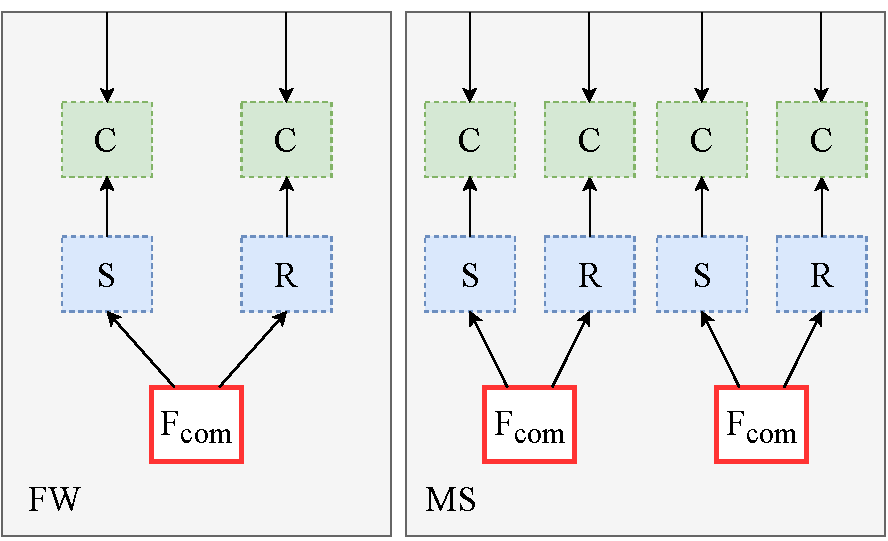
\includegraphics[scale=0.5]{figures/multisession.pdf}
%\caption{The multisession extension of \Fcom (right) with only two instances, creates the same processes $S$ and $R$ (offering the session typed channel to \Fcom) for every created instance. A communicator per session buffers messages for the $S$ and $R$ processes to consume and forward along their session-typed channel to \Fcom.}
%\label{fig:multisession}
%\end{figure}

%As a generic construction provided by NomosUC, the multisession operator requires some code generation but only to accept an arbitrary number of virtual token types if the underlying \F simulators other processes. 
%Furthermore, similar to the functionality wrapper, the multisession operator constructs the processes around \F in the same way and spawns them on-demand.
%The process definition for $!\F_\msf{com}$ is shown in Figure \ref{lst:bangf} accepting two token types: the real token type $K$ and the virtual token type $K_1$ for instances of $\F_\msf{com}$.
%
%\begin{figure}
%\begin{lstlisting}[basicstyle=\footnotesize\BeraMonottFamily, frame=single, mathescape]
%$\tb{proc}$ bangF[K,K1][p2f,...] :
%  (k: $\tgr{Int}$), (rng: [Bit]), (sid: session[a]), 
%  ($\$$p: P2MS[p2f][f2p]) |- ($\$$ch: 1) =
%\end{lstlisting}
%\caption{The type definition for the multisession operator for functionalities and the correspond message type and import parameters. The operator for protocol parties is identical in code but differens in that the parameters to the \texttt{P2MS} type are for \texttt{Z2P} interaction.}
%\label{lst:bangf}
%\end{figure}


%\begin{proof}
%A \textit{well-resource-typed} \F guarantees a polynomial $T_{\F}$ bounding its execution.
%In the worse-case, the multisession operator must spawn a new instance of $\F$ an every activation. 
%Let $N_{\F}$ denote the total number of instances (and, hence, number of activations) of $\F$ created by the operator.
%Note that $N_{\F}$ is polynomial in the security parameter $k$ for all well-typed environments, protocols, and adversary.
%Therefore, there always exists a bounding polynomial to bound a polynomial number of simulated instances of \F.
%The polynomial can be given as:
%$$ P_{!\F}(n) = N_{\F} P_{\F}(n) + \mathcal{O}(N_{\F}) $$
%where the $\mathcal{O}(N_{\F})$ is due to the overhead of maintaining and accessing the set of all instances.
%
%Similarly, \F being \textit{well-resource-typed} ensures a valid token context for all processes it may simulate. 
%Therefore, it is clear that there exists a global connecting poltnomial $f$ that ensures a valid token context for $!\F$.
%\end{proof}


%\begin{figure}
%\begin{lstlisting}[basicstyle=\small\BeraMonottFamily, mathescape, frame=single]
%$\yo{type}$ p2bFmsg[a] = P2bF of ssid ^ a ;
%$\yo{type}$ p2bbFmsg[a] = P2bbF of ssid ^ ssid ^ a ;
%$\tg{(* z2p : comm[z2pmsg[p2bbf[a]]] *)}$
%$\tg{(* p2f : comm[p2fmsg[P2bf[a]]] *)}$
%pid = recv $\$$z2p ;
%m = recv $\$$z2p ;
%case m (
%  P2bbF(ssid1, ssid2, m) =>
%    send $\$$p2f P2bF(ssid1 + ssid2, m) ;
%)
%\end{lstlisting}
%\caption{The \textit{squash protocol} accepts a message intended intended for $!!\F$ of type \inline{P2MS[p2ms[a]][ms2p[b]]}, i.e. of the form $(\msf{ssid}_1, (\msf{ssid}_1, msg))$.
%It ``flattens'' it into a single $\msf{ssid}_3 = \msf{ssid}_1 + \msf{ssid}_2$ that can be passed to $!\F$. The result is the same number of instances of \F but behind only a single $!$ operator.}
%\label{fig:squash}
%\end{figure}

We can now, finally, conclude with full composition in Theorem~\ref{thm:composition}.
The proof follows directly from Theorems~\ref{thm:singlecomp}, \ref{thm:functor}, and a squash protocol described in Appendix~\ref{app:ms} which squashes multiple sessions of \F into one. 

\begin{proof}
By Theorem~\ref{thm:singlecomp} we have that $\F_1 \xrightarrow{\pi} \F_2$. If we combine this result with Theorem~\ref{thm:functor} we can conclude that $!!\F_1 \xrightarrow{\rho \circ !\pi} !\F_3$. 
Finally we can squash one $!$ operator with Theorem~\ref{thm:squash} (in Appendix~\ref{app:ms} to get $!\F_1 \xrightarrow{\rho \circ !\pi \circ \m{squash}} \F_3$.
\end{proof}


